\clearpage
\cleardoublepage

\chapter{数据集处理}

\section{引言}

机器学习模型的质量从根本上受限于其训练数据的质量俗话说："垃圾进，垃圾出。"本章涵盖神经网络训练数据准备的端到端流水线：收集、标注、划分、增强、加载、归一化，以及日益重要的数据质量和版本管理考量。

虽然讨论的技术广泛适用，但我们特别关注不同数据模态——图像、文本和音频——的独特处理要求。

\section{数据收集}

任何机器学习系统的基础是高质量数据。数据集决定了模型所能达到的性能上限。

\subsection{数据来源}

数据可以从多个来源获取，每个来源都有其质量和成本权衡：

\begin{itemize}
    \item \textbf{公共数据集：}策划的基准数据集（ImageNet、COCO、GLUE、SQuAD）提供标准化评估，但可能与目标分布不匹配。
    \item \textbf{网页抓取：}从网站自动收集数据以低成本提供大量数据，但需要仔细去重和质量过滤。
    \item \textbf{传感器：}摄像头、麦克风、医学成像设备、加速度计产生丰富数据，但需要仔细校准和预处理。
    \item \textbf{人工标注：}专家标注提供高质量的真实标签，但成本高且速度慢。众包平台（Amazon Mechanical Turk、Scale AI）以规模换速度，牺牲标注质量。
    \item \textbf{合成数据：}从模拟或生成模型生成的数据可以扩充有限的真实数据，在医学成像和机器人技术中特别有价值。
\end{itemize}

\subsection{数据质量标准}

高质量数据集共享几个特性：

\begin{enumerate}
    \item \textbf{正确性：}标签准确反映真实标签。错误引入偏差并限制模型性能上限。
    \item \textbf{一致性：}标注指南明确无歧义，标注者统一应用。
    \item \textbf{代表性：}数据集分布与目标部署领域匹配。在日光图像上训练的模型在夜间场景会失败。
    \item \textbf{平衡性：}类别频率和难度级别适合任务。严重不平衡需要特殊处理。
    \item \textbf{去重：}近似重复的样本膨胀了有效数据集大小并导致训练-测试泄露。
\end{enumerate}

\section{数据标注}

标签实现监督学习。标注策略取决于任务类型。

\subsection{标注类型}

\begin{figure}[htbp]
    \centering
    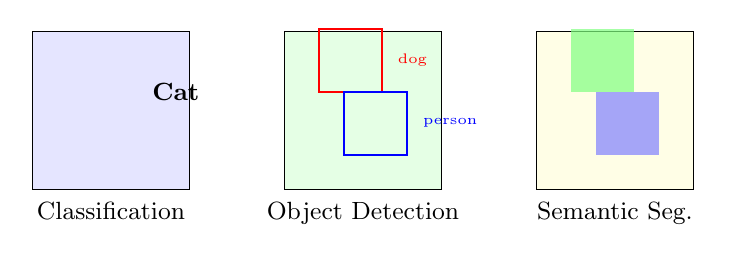
\begin{tikzpicture}[scale=0.8]
        % Classification
        \node[draw, rectangle, minimum width=2cm, minimum height=2cm, fill=blue!10] (cls) at (0,0) {};
        \node[below, font=\small] at (0, -1.3) {Classification};
        \node[right, font=\small] at (0.5, 0.3) {\textbf{Cat}};
        
        % Detection
        \node[draw, rectangle, minimum width=2cm, minimum height=2cm, fill=green!10] (det) at (4,0) {};
        \draw[red, thick] (3.3, 0.3) rectangle (4.3, 1.3);
        \draw[blue, thick] (3.7, -0.7) rectangle (4.7, 0.3);
        \node[below, font=\small] at (4, -1.3) {Object Detection};
        \node[right, red, font=\tiny] at (4.4, 0.8) {dog};
        \node[right, blue, font=\tiny] at (4.8, -0.2) {person};
        
        % Segmentation
        \node[draw, rectangle, minimum width=2cm, minimum height=2cm, fill=yellow!10] (seg) at (8,0) {};
        \fill[green!50, opacity=0.7] (7.3, 0.3) rectangle (8.3, 1.3);
        \fill[blue!50, opacity=0.7] (7.7, -0.7) rectangle (8.7, 0.3);
        \node[below, font=\small] at (8, -1.3) {Semantic Seg.};
    \end{tikzpicture}
    \caption{标注粒度：从图像级标签到像素级分割掩码。}
    \label{fig:annotation_types}
\end{figure}

\begin{itemize}
    \item \textbf{分类：}每张图像一个标签（如猫vs狗）。最简单的标注任务，容易出现模糊情况。
    \item \textbf{多标签分类：}每张图像多个标签（如"海滩、日落、人"）。每个标签是独立的二元决策。
    \item \textbf{目标检测：}带类别标签的边界框。每个框指定一个区域及其类别。
    \item \textbf{语义分割：}像素级类别标签。每个像素被分配一个类别（或"背景"）。
    \item \textbf{实例分割：}区分同类的不同个体（如每个人是一个单独的实例）。
    \item \textbf{关键点检测：}感兴趣点（面部标志、人体关节、车辆检测点）。
\end{itemize}

\subsection{标注工具}

\begin{itemize}
    \item \textbf{LabelImg：}用于边界框标注的开源工具。快速且轻量级。
    \item \textbf{CVAT：}计算机视觉标注工具，支持视频、图像和文本标注，具有协作功能。
    \item \textbf{Supervisely：}功能齐全的平台，带AI辅助标注（用现有模型预标注）。
    \item \textbf{Amazon Mechanical Turk：}大规模众包人工标注。通过共识/黄金问题进行质量控制。
    \item \textbf{Label Studio：}高度可配置的开源标注工具，支持多种数据类型。
\end{itemize}

\section{数据划分}

正确的数据划分对于获得模型性能的无偏估计至关重要。

\subsection{基本划分}

\begin{itemize}
    \item \textbf{训练集：}用于更新模型参数的样本。通常占数据的70-90\%。
    \item \textbf{验证集：}用于超参数调整和模型选择。不用于训练。
    \item \textbf{测试集：}用于最终评估。不得影响任何训练决策。
\end{itemize}

\textbf{典型比例：}
\begin{itemize}
    \item 小数据集（$<$10K）：70/10/20或80/10/10（训练/验证/测试）
    \item 中等数据集（10K-1M）：80/10/10或85/5/10
    \item 大数据集（$>$1M）：98/1/1可能足够，但确保测试集足够大以获得可靠估计
\end{itemize}

\begin{note}[测试集泄露]
永远不要将测试集用于训练期间的任何决策。这包括选择超参数、选择架构或早停阈值。这样做会导致过度拟合测试集和不可靠的性能估计。测试集应该"锁起来"直到最终评估。
\end{note}

\subsection{分层划分}

当类别分布不平衡时，随机划分可能产生不具代表性的划分。分层划分保持每个划分中的类别比例：

\begin{verbatim}
from sklearn.model_selection import train_test_split
X_train, X_test, y_train, y_test = train_test_split(
    X, y, test_size=0.2, stratify=y
)
\end{verbatim}

对于多标签分类，分层更复杂。一种方法是将每个标签组合视为一个单独的类别，尽管这可能导致罕见的组合。或者，迭代标签并平衡每个。

\subsection{交叉验证}

对于有限数据的稳健评估，$K$折交叉验证提供更可靠的估计：

\begin{algorithm}[H]
\caption[$K$折交叉验证]{$K$折交叉验证}
\begin{enumerate}
    \item 打乱数据并分成$K$个相等的折
    \item 对于$i = 1, 2, \ldots, K$：
    \begin{enumerate}
        \item 在折$\{1, 2, \ldots, K\} \setminus \{i\}$上训练
        \item 在折$i$上验证
    \end{enumerate}
    \item 报告验证指标的平均值和标准差
\end{enumerate}
\end{algorithm}

常见值：$K = 5$（对于中等数据）或$K = 10$（对于小数据，较大方差减少）。分层$K$折保持每个折中的类别比例。

\section{数据增强}

数据增强通过对现有样本应用随机变换人为增加数据集大小，在不需要额外数据收集的情况下提高泛化能力。

\subsection{图像增强}

\begin{figure}[htbp]
    \centering
    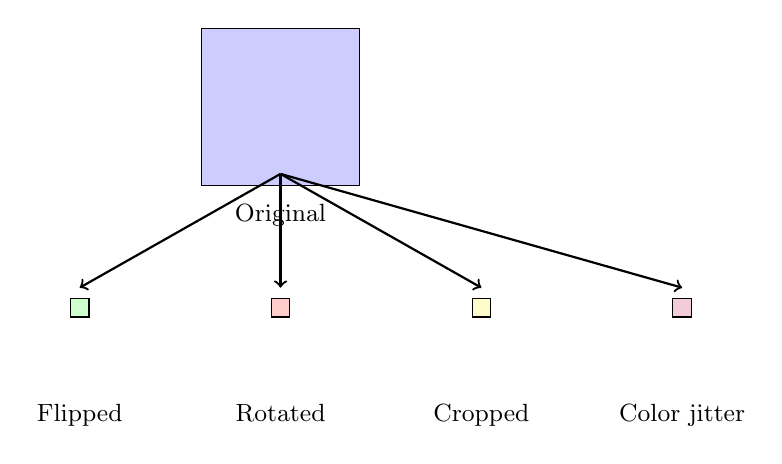
\begin{tikzpicture}[scale=0.85]
        % Original
        \node[draw, rectangle, minimum width=2cm, minimum height=2cm, fill=blue!20] (orig) at (0,0) {};
        \node[below, font=\small] at (0, -1.3) {Original};
        
        % Augmentations
        \node[draw, rectangle, fill=green!20] at (-3, -3) {};
        \node[below, font=\small] at (-3, -4.3) {Flipped};
        
        \node[draw, rectangle, fill=red!20] at (0, -3) {};
        \node[below, font=\small] at (0, -4.3) {Rotated};
        
        \node[draw, rectangle, fill=yellow!20] at (3, -3) {};
        \node[below, font=\small] at (3, -4.3) {Cropped};
        
        \node[draw, rectangle, fill=purple!20] at (6, -3) {};
        \node[below, font=\small] at (6, -4.3) {Color jitter};
        
        % Arrows
        \foreach \x in {-3, 0, 3, 6} {
            \draw[->, thick] (0, -1.0) -- (\x, -2.7);
        }
    \end{tikzpicture}
    \caption{图像增强示例：水平翻转、旋转、随机裁剪和颜色抖动。}
    \label{fig:augmentation}
\end{figure}

常见几何增强：
\begin{itemize}
    \item \textbf{旋转：}随机角度旋转（如$\pm 15^\circ$）。应在保持标签的范围内。
    \item \textbf{翻转：}水平翻转（左右镜像）。对于大多数分类任务是安全的，但不适用于文本或不对称物体。
    \item \textbf{随机裁剪：}裁剪到较小区域，然后调整大小到原始大小。强制尺度不变性。
    \item \textbf{缩放：}随机缩放（放大/缩小）。与不同裁剪比例的随机裁剪效果相同。
    \item \textbf{平移：}在$x$和$y$方向上的随机平移。等价于非对称裁剪。
\end{itemize}

颜色增强：
\begin{itemize}
    \item \textbf{颜色抖动：}对亮度、对比度、饱和度和色调的随机调整。
    \item \textbf{高斯噪声：}注入像素级高斯噪声以提高鲁棒性。
    \item \textbf{Cutout/随机擦除：}随机遮挡矩形区域。迫使模型使用分布式特征。
    \item \textbf{灰度/RGB排列：}对于多通道图像。
\end{itemize}

Mixup和CutMix增强将样本混合在一起：

\subsection{Mixup：样本的凸组合}

Mixup \cite{zhang2018mixup}通过在样本对之间线性插值创建虚拟训练样本：
\begin{align}
\tilde{\mathbf{x}} &= \lambda \mathbf{x}_i + (1 - \lambda)\mathbf{x}_j \\
\tilde{\mathbf{y}} &= \lambda \mathbf{y}_i + (1 - \lambda)\mathbf{y}_j
\end{align}
其中$\lambda \sim \text{Beta}(\alpha, \alpha)$，$\alpha \in (0, \infty)$。混合系数$\lambda$控制每个样本的相对权重。

\textbf{Mixup为什么有效：}
\begin{enumerate}
    \item \textbf{正则化：}模型看到平滑的决策边界，防止过度自信
    \item \textbf{数据清理：}将噪声标签与干净标签混合稀释标签噪声
    \item \textbf{更好的校准：}对混合输入的预测鼓励更软的目标
    \item \textbf{标签平滑效果：}对于分类，即使$y_i, y_j$是独热的，$\tilde{y}$也是类上的概率分布
\end{enumerate}

对于具有独热标签$\mathbf{y}_i, \mathbf{y}_j \in \{0,1\}^K$的$K$类分类问题，混合标签$\tilde{\mathbf{y}}$是类上的概率分布。Mixup损失变为：
\begin{equation}
\mathcal{L}_{\text{mixup}} = -\sum_{k=1}^{K} \tilde{y}_k \log \hat{y}_k = -\lambda \sum_k y_{i,k} \log \hat{y}_k - (1-\lambda) \sum_k y_{j,k} \log \hat{y}_k
\end{equation}

这等价于最小化预测与两个独热标签混合之间的交叉熵。

\subsection{CutMix：粘贴补丁}

CutMix \cite{yun2019cutmix}将一个图像的矩形区域粘贴到另一个图像中，而不是混合：
\begin{align}
\tilde{\mathbf{x}} &= \mathbf{x}_i \odot \mathbf{M} + \mathbf{x}_j \odot (1 - \mathbf{M}) \\
\tilde{\mathbf{y}} &= \lambda \mathbf{y}_i + (1 - \lambda)\mathbf{y}_j
\end{align}
其中$\mathbf{M} \in \{0,1\}^{H \times W}$是二进制掩码，$\lambda = \frac{\text{area}(\mathbf{M})}{HW}$。

\textbf{CutMix vs. Mixup：}CutMix保留图像的像素级特性（边界处无模糊），同时仍提供Mixup的正则化优势。矩形掩码在区域之间提供清晰对比，这可以帮助模型学习局部特征。

\begin{code}
    \captionof{listing}{PyTorch中的Mixup和CutMix}
    \label{code:mixup_cutmix}
\begin{lstlisting}[language=python]
import torch
import numpy as np

def mixup_data(x, y, alpha=1.0):
    """Returns mixed inputs, pairs of targets, and lambda."""
    if alpha > 0:
        lam = np.random.beta(alpha, alpha)
    else:
        lam = 1
    
    batch_size = x.size(0)
    index = torch.randperm(batch_size).to(x.device)
    
    mixed_x = lam * x + (1 - lam) * x[index, :]
    y_a, y_b = y, y[index]
    return mixed_x, y_a, y_b, lam

def mixup_criterion(criterion, pred, y_a, y_b, lam):
    return lam * criterion(pred, y_a) + (1 - lam) * criterion(pred, y_b)

def cutmix_data(x, y, alpha=1.0):
    """CutMix: Cuts and pastes patches between images."""
    if alpha > 0:
        lam = np.random.beta(alpha, alpha)
    else:
        lam = 1
    
    batch_size = x.size(0)
    index = torch.randperm(batch_size).to(x.device)
    
    # Get bounding box
    W = x.size(3); H = x.size(2)
    cut_rat = np.sqrt(1. - lam)
    cut_w = int(W * cut_rat); cut_h = int(H * cut_rat)
    
    cx = np.random.randint(W)
    cy = np.random.randint(H)
    bbx1 = np.clip(cx - cut_w // 2, 0, W)
    bby1 = np.clip(cy - cut_h // 2, 0, H)
    bbx2 = np.clip(cx + cut_w // 2, 0, W)
    bby2 = np.clip(cy + cut_h // 2, 0, H)
    
    x[:, :, bby1:bby2, bbx1:bbx2] = x[index, :, bby1:bby2, bbx1:bbx2]
    lam = 1 - ((bbx2 - bbx1) * (bby2 - bby1) / (W * H))
    
    y_a, y_b = y, y[index]
    return x, y_a, y_b, lam
\end{lstlisting}
\end{code}

\subsection{高级增强策略}

而不是手动设计增强，自动化方法搜索最优增强策略：

\begin{itemize}
    \item \textbf{AutoAugment} \cite{cubuk2019autoaugment}：从CIFAR-10/CIFAR-100学习的策略。发现的策略可以很好地迁移到其他数据集，但计算成本高。
    \item \textbf{RandAugment} \cite{cubuk2020randaugment}：简化的搜索空间，只有两个参数（幅度、操作数量）。以少得多的计算几乎匹配AutoAugment。
    \item \textbf{TrivialAugment Wide} \cite{muller2023torchvision}：无需搜索。以随机幅度应用随机选择的增强。出人意料地有效且简单。
    \item \textbf{测试时增强（TTA）：}在推理时应用增强并平均预测。以$K\times$推理时间为代价提供免费的精度提升（通常1-2\%）。
\end{itemize}

\section{文本数据处理}

文本数据需要与图像根本不同的预处理，围绕分词概念展开。

\subsection{分词}

分词将原始文本字符串转换为模型可以处理的离散令牌序列（词ID或子词ID）。

\begin{table}[ht]
    \centering
    \caption{分词策略}
    \begin{tabular}{L{3cm} L{4cm} L{4cm}}
        \toprule
        \textbf{策略} & \textbf{示例} & \textbf{优点/缺点} \\
        \midrule
        词级 & ``hello world'' $\to$ [12, 45] & 简单；大词表，OOV问题 \\
        字符级 & ``hello'' $\to$ [104, 101, 108, 108, 111] & 小词表；长序列，无语义 \\
        BPE & ``unhappiness'' $\to$ [``un'', ``happy'', ``ness''] & 良好的平衡；从数据学习 \\
        WordPiece & BERT分词器 & 类似BPE；掩码LM训练 \\
        SentencePiece & 统一分词 & 语言无关；处理任意文本 \\
        \bottomrule
    \end{tabular}
\end{table}

\subsection{字节对编码（BPE）}

BPE \cite{sennrich2016neural}是现代LLM中最广泛使用的子词分词算法。它通过迭代合并语料库中最频繁的相邻字节/字符对来构建词表：

\begin{enumerate}
    \item 从所有单个字符加上词尾令牌开始词表
    \item 计算语料库中所有相邻对
    \item 将最频繁的对合并为单个令牌
    \item 对$N$次合并操作重复（其中$N$是超参数）
\end{enumerate}

词表大小是一个关键超参数：更大的词表将更多单词表示为单个令牌（推理更快）但需要更多嵌入和更高的内存占用。

对于大小为$V$的词表，BPE需要$\mathcal{O}(V)$空间。现代LLM通常使用$V = 30{,}000$--$100{,}000$个令牌。

\section{音频数据处理}

音频数据通常作为频谱图或梅尔频谱图处理。

\subsection{频谱图计算}

短时傅里叶变换（STFT）将时域信号$x[t]$转换为时频表示：

\begin{equation}
X[m, k] = \sum_{n=0}^{N-1} x[n] w[n] e^{-j 2\pi kn/N}
\end{equation}
其中$w[n]$是窗口函数（Hann或Hamming），$N$是FFT大小。

\textbf{梅尔频谱图}将频率映射到梅尔刻度，近似人类听觉感知：
\begin{equation}
f_{\text{mel}} = 2595 \log_{10}\!\left(1 + \frac{f_{\text{Hz}}}{700}\right)
\end{equation}

\section{数据归一化}

归一化标准化输入特征，通过确保所有输入在相似尺度上来稳定训练。

\subsection{图像归一化}

对于RGB图像，像素值$x \in [0, 255]$通常归一化到$[0, 1]$或标准化到零均值和单位方差：

\begin{equation}
x_{\text{norm}} = \frac{x - \mu}{\sigma}
\end{equation}

ImageNet归一化参数：
\begin{itemize}
    \item 均值：$[\,0.485,\, 0.456,\, 0.406\,]$
    \item 标准差：$[\,0.229,\, 0.224,\, 0.225\,]$
\end{itemize}

这些值是从ImageNet训练集计算的。对于自定义数据集，计算特定于数据集的统计量：

\begin{lstlisting}[language=python]
loader = DataLoader(dataset, batch_size=32)
mean = torch.zeros(3); std = torch.zeros(3)
for images, _ in loader:
    mean += images.mean(dim=[0, 2, 3])
    std += images.std(dim=[0, 2, 3])
mean /= len(loader.dataset)
std /= len(loader.dataset)
\end{lstlisting}

注意：使用预训练模型时，始终使用模型训练时使用的统计量，即使它们对您的数据不是最佳的。

\section{数据加载}

高效的数据加载防止GPU饥饿并最大化训练吞吐量。

\begin{code}
    \captionof{listing}{PyTorch中的高效数据加载}
    \label{code:dataloader}
\begin{lstlisting}[language=python]
from torch.utils.data import DataLoader, Dataset

class ImageDataset(Dataset):
    def __init__(self, data, labels, transform=None):
        self.data = data
        self.labels = labels
        self.transform = transform
    
    def __len__(self):
        return len(self.data)
    
    def __getitem__(self, idx):
        image = self.data[idx]
        label = self.labels[idx]
        if self.transform:
            image = self.transform(image)
        return image, label

train_loader = DataLoader(
    train_dataset,
    batch_size=32,
    shuffle=True,         # Important for SGD convergence
    num_workers=4,        # Parallel data loading
    pin_memory=True,      # Faster GPU transfer (CUDA pinning)
    drop_last=True,       # Consistent batch sizes
    persistent_workers=True  # Keep workers alive between epochs
)

# Prefetch next epoch while current epoch trains
val_loader = DataLoader(
    val_dataset,
    batch_size=64,
    shuffle=False,         # No need to shuffle validation
    num_workers=4,
    pin_memory=True
)
\end{lstlisting}
\end{code}

\begin{properties}[DataLoader优化]
\begin{itemize}
    \item \textbf{num\_workers}：更多worker = 更快加载，但太多会导致CPU-GPU争用。好的起点是4-8。
    \item \textbf{pin\_memory}：固定CPU内存以便更快传输到GPU（避免额外的内存复制）。
    \item \textbf{drop\_last}：删除最后一个不完整批次以避免变化的批次大小（对于批量归一化尤其重要）。
    \item \textbf{persistent\_workers}：在轮次之间保持worker进程存活，减少每轮启动开销。
\end{itemize}
\end{properties}

\section{处理数据不平衡}

类别不平衡在现实世界数据集中普遍存在，如果不解决，会严重降低模型性能。

\subsection{不平衡比例}

常见不平衡比例：
\begin{itemize}
    \item 轻度（1:10到1:100）：标准医学成像、异常检测
    \item 严重（1:100到1:1000）：欺诈检测、罕见疾病诊断
    \item 极端（$<$1:1000）：科学应用（粒子物理、天文学）
\end{itemize}

\subsection{不平衡数据技术}

\begin{enumerate}
    \item \textbf{加权损失函数：}为少数类分配更高的损失权重：
    \begin{equation}
    \mathcal{L}_{\text{weighted}} = -\sum_{k=1}^{K} w_k \cdot y_k \log \hat{y}_k
    \end{equation}
    其中$w_k = N / (K \cdot N_k)$，$N_k$是类$k$中的样本数。
    
    \item \textbf{过采样少数类：}复制少数样本或生成合成样本（表格数据的SMOTE）。
    
    \item \textbf{欠采样多数类：}随机删除多数类样本以平衡数据集。
    
    \item \textbf{Focal Loss} \cite{lin2017focal}：降低简单样本的权重，将训练重点放在难样本上：
    \begin{equation}
    \mathcal{L}_{\text{focal}} = -(1 - p_t)^\gamma \log p_t
    \end{equation}
    其中$p_t$是模型对真实类别的预测概率，$\gamma \geq 0$控制降权强度。详见第3章的详细推导。
\end{enumerate}

\section{数据质量与版本管理}

随着数据集在重要性和复杂性上的增长，系统的数据管理变得必不可少。

\subsection{数据版本管理}

数据版本管理跟踪数据集随时间的变化，实现：
\begin{itemize}
    \item 可重复性：不同时间点使用完全相同的数据进行训练
    \item 溯源跟踪：理解哪个模型在哪个版本的数据上训练
    \item 回滚：如果发现问题则回滚到以前的数据版本
    \item 实验比较：测试关于数据质量的假设
\end{itemize}

像\textbf{DVC}（数据版本控制）这样的工具扩展Git以处理大文件和ML流水线：
\begin{verbatim}
dvc init
dvc add data/
git add data.dvc
git commit -m "Add dataset v1"
# Later, update and version:
dvc add data/
git add data.dvc
git commit -m "Update to dataset v2"
\end{verbatim}

DVC将实际数据存储在远程存储（S3、GCS、Azure Blob）中，而Git跟踪元数据和哈希，实现高效协作。

\subsection{数据溯源}

理解数据溯源回答：这个样本从哪里来？谁标注的？什么时候添加的？

关键溯源元数据：
\begin{itemize}
    \item 来源URL或收集方法
    \item 收集/标注时间戳
    \item 标注者ID及其资质
    \item 标注质量分数（如果使用共识标注）
    \item 处理流水线版本（应用的增强、过滤器）
\end{itemize}

此元数据对于调试模型失败、审计偏差以及在高风险领域（医疗保健、金融、法律）满足监管要求至关重要。

\section{评估指标}

虽然第3章涵盖了损失函数，但本节讨论特定任务的评估指标。

\subsection{分类指标}

\begin{itemize}
    \item \textbf{准确率：}正确预测的比例。简单但对不平衡数据有误导。
    \item \textbf{精确率、召回率、F1：}对于二分类：
    \begin{align}
    \text{精确率} &= \frac{TP}{TP + FP} \quad \text{（预测为正的中有多少正确？）} \\
    \text{召回率} &= \frac{TP}{TP + FN} \quad \text{（实际为正的中找到多少？）} \\
    F_1 &= \frac{2 \cdot \text{精确率} \cdot \text{召回率}}{\text{精确率} + \text{召回率}}
    \end{align}
    \item \textbf{宏/微F1：}宏平均先计算每类F1再平均；微平均先跨类计算TP/FP/FN再计算F1。
    \item \textbf{AUC-ROC：}ROC曲线下面积。与阈值无关；衡量排序质量。
\end{itemize}

\subsection{分割指标}

\begin{itemize}
    \item \textbf{交并比（IoU）：} $\text{IoU} = \frac{|A \cap B|}{|A \cup B|}$
    \item \textbf{Dice系数：} $\text{Dice} = \frac{2|A \cap B|}{|A| + |B|} = \frac{2 \cdot \text{IoU}}{1 + \text{IoU}}$
    \item \textbf{像素准确率：}正确分类像素的比例。
\end{itemize}

注意：IoU和Dice相关：$\text{Dice} = \frac{2 \cdot \text{IoU}}{1 + \text{IoU}}$，所以优化一个近似优化另一个。

\section{章节小结}

\begin{enumerate}
    \item 数据质量是模型性能的基础；即使是最好的架构也无法克服糟糕的数据
    \item 正确的训练/验证/测试划分防止泄露并提供无偏的性能估计
    \item 交叉验证（$K$折）在数据有限时提供稳健估计
    \item 数据增强通过随机变换人为扩展有效数据集
    \item Mixup和CutMix通过凸组合或补丁粘贴创建虚拟训练样本，提供强正则化
    \item 文本数据需要在模型输入前进行分词（BPE、WordPiece）
    \item 归一化通过标准化输入尺度稳定训练
    \item 带多个worker和固定内存的高效数据加载最大化GPU利用率
    \item 类别不平衡需要通过加权损失或focal loss进行特殊处理
    \item 数据版本管理和溯源跟踪对于可重复的ML研究和生产系统必不可少
    \item 评估指标应匹配下游任务要求；对于不平衡或多类问题，仅准确率是不够的
\end{enumerate}

\section{延伸阅读}

\begin{itemize}
    \item \cite{goodfellow2016deep} --- 深度学习章节，数据处理部分
    \item \cite{sennrich2016neural} --- 带有子词单元的神经机器翻译
    \item \cite{lin2017focal} --- 密集目标检测的Focal Loss
    \item \cite{chollet2017deep} --- Python深度学习，第4章预处理流水线
    \item \cite{zhang2018mixup} --- mixup：超越经验风险最小化
    \item \cite{cubuk2019autoaugment} --- AutoAugment：从数据学习增强策略
    \item \cite{yun2019cutmix} --- CutMix：训练强分类器与可定位特征的正则化策略
    \item \cite{cubuk2020randaugment} --- RandAugment：实用自动化数据增强与减少的搜索空间
    \item DVC文档：\url{https://dvc.org/} --- ML项目的数据版本控制
\end{itemize}

\section{练习题}

\begin{enumerate}
    \item \textbf{数据泄露：}在图像分类或表格ML流水线中给出两个数据泄露的例子。为什么泄露可能使验证准确率误导性地高？

    \item \textbf{划分策略：}您有12,000个标注样本和5个类别，中等不平衡。设计一个训练/验证/测试划分策略，并解释是否需要分层。

    \item \textbf{Mixup标签：}如果两个具有独热标签$y_a$和$y_b$的图像以$\lambda = 0.3$组合，写出用于训练的新目标标签。

    \item \textbf{增强策略：}比较AutoAugment、RandAugment和TrivialAugment Wide。当策略搜索的计算受限时，哪个最容易部署？

    \item \textbf{分词：}解释为什么子词分词（BPE/WordPiece）通常比纯词级分词对开放词汇NLP效果更好。

    \item \textbf{输入流水线效率：}为什么多个data-loader worker和固定内存通常可以提高GPU利用率？什么时候它们可能无法帮助？
\end{enumerate}
